%! Licence = CC BY-NC-SA 4.0

%! Author = gianfluetsch
%! Date = 30. Dez 2021
%! Project = cydef_summary


\section{Mimikatz}

\subsection{Windows Credential Management}

\subsubsection{Logon Session}
Windows erstellt bei erfolgreicher Authentifizierung eine Logon Session
\begin{itemize}
    \item Benutzeranmeldeinformationen werden in lsass.exe gespeichert
    \item Betriebssystem kann sie später für SSO bei anderen Diensten verwenden
    \item Benutzeranmeldeinformationen sind an Authentifizierungspakete innerhalb der Logon Session gebunden:
    \begin{itemize}
        \item NTLM-Hashes
        \item Kerberos-Tickets/Keys
        \item Passwörter im Klartext
    \end{itemize}
\end{itemize}

\subsubsection{Tokens}
Aktueller Sicherheitskontext eines Prozesses/Threads
\begin{itemize}
    \item Thread/Prozess verwendet ein Token im Namen eines Benutzers
    \item Token sind an eine Logon Session gebunden und bestimmen, wie das Credential verwendet wird
\end{itemize}

\subsubsection{Logon Session Types}
\begin{itemize}
    \item \textbf{Network Logons} (Type 3):\\
    Clients beweist, dass Anmeldedaten hat, \underline{senden aber nicht}! (NTLM-Challenge/Response $\rightarrow$ Pass-the-Hash auf SMB-Dateiserver)
    \item \textbf{Non-Network Logon} (Interactive/NetworkCleartext):\\
    Anmeldedaten \underline{werden zum Server gesendet} und \underline{in LSASS Memory} \underline{gespeichert} (z.B. RDP interactive logon)
\end{itemize}
Mit \underline{Network Logon} können \underline{keine} Credentials gestohlen werden!

\subsubsection{Token Types \& Impersonation}
\textbf{Primary Token}:\\
ein Prozess-Token (Sicherheitskontext des mit dem Prozess verbundenen Benutzerkontos)\\
\textbf{Impersonating Token}:\\
ein Thread-Token (um andere Token in Client/Server-Szenarien zu verkörpern)\\
\textbf{Impersonating Levels}:
\begin{itemize}
    \item Anonymous\\
    Entfernter Server kann einen Client nicht identifizieren, der Thread agiert als anonymer Benutzer.
    \item Identification\\
    Entfernte Server kann den Benutzer identifizieren, aber nicht ,,impersonaten``
    \item Impersonation\\
    Der entfernte Server kann den Client über eine Computergrenze hinweg identifizieren und sich als dieser ausgeben (Netzwerkanmeldung beim Server)
    \item Delegation\\
    Der Server kann sich über mehrere Grenzen hinweg als Client ausgeben und Anrufe im Namen des Clients tätigen (bekannt als Kerberos ,,double hop``)
\end{itemize}
\textbf{Bemerkung:}
Wird ein \underline{Impersonation Token} mit \underline{Anonymous} oder \underline{Identification Level} gestohlen, kann es \underline{nicht} für \underline{remote authentifikation} verwendet werden! \\
Wird ein \underline{Impersonation oder Process Token} mit \underline{Impersonation} \underline{Delegation Level} gestohlen, \underline{kann es} für \underline{remote authentifikation} verwendet werden (falls korrespondierende Logon Session credentials hat)!

\subsubsection{Mimikatz und Tokens}
Mimikatz kann mit existierenden Prozess und Thread Token interagieren:
\begin{itemize}
    \item Abgreifen
    \item Imitieren
\end{itemize}

\subsubsection{Douple-Hop Problem}
Wenn Code mit WMI oder WinRM aus der Ferne ausgeführt wird, erhalten man ein Token, das an eine Network Logon Session gebunden ist $\rightarrow$ Anmeldeinformationen werden nicht tatsächlich an den Remote-Host gesendet.\\
Von diesem kompromittierten Host aus kann man sich \underline{nicht bei anderen Ressourcen im Netzwerk authentifizieren}!\\
\textbf{Workaround:}
\begin{itemize}
    \item Anderes Token verwenden, das auf eine Non-Network Logon Session verweist:
    \begin{itemize}
        \item Stehlen eines Tokens
        \item Einschleusen in einen anderen Prozess
    \end{itemize}
    \item Erstellen eines neuen Tokens, das auf eine Non-Network Logon Session mit gestohlenen Anmeldedaten verweist
    \item Anmeldeinformationen in die aktuelle Anmeldesitzung laden (z.B. pass-the-ticket)
\end{itemize}

\subsection{Mimikatz}

\subsubsection{Übersicht}
\begin{itemize}
    \item Post-Exploitation-Tool zum Abrufen von Anmeldedaten
    \item Nicht verwendet werden um lokaler Admin zu werden
    \item Erfordert lokale Admin-Rechte
    \item Versucht Domain-Admin Credentials auszulesen, welche lokal gespeichert/gecached sind.
    \item Abrufen von Anmeldeinformationen aus dem LSASS-Speicher oder SAM-Dateien:
    \begin{itemize}
        \item Klartext-Passwörter $\rightarrow$  abhängig von Windows-Version und GPO-Einstellungen
        \item NTLM-Hashes
        \item Kerberos-Tickets
    \end{itemize}
    \item Kann Pass-the-Hash-Angriffe durchführen
    \item Kann Pass-the-Ticket-Angriffe durchführen
    \item Kann benutzerdefinierte golden Tickets erstellen (für Kerberos-Authentifizierung)
\end{itemize}

\subsubsection{Extract local credentials from SAM}
Das lsadump Modul ermöglicht die Interaktion mit der local security authority (LSA), um lokale Anmeldeinformationen von einem Rechner zu extrahieren.

\subsubsection{Dumping Credentials from LSASS Memory}
Das sekurlsa Modul ermöglicht die Interaktion mit der local security authority subsytem process memory (LSASS.exe)
Die Interaktion mit dem Speicher von lsass.exe ist der Feind Nr. 1 für Abwehrprodukte! Speicher von lsass.exe sollte überwachen werden.

\subsubsection{The output}
Für jede Anmeldesitzung zählt Mimikatz die Anmeldedaten in jedem Authentifizierungspaket auf:\\
Thread/Process $\rightarrow$ Token $\rightarrow$ Logon Session $\rightarrow$ Auth Package $\rightarrow$ Credential

\vfill
$ $
\columnbreak

\subsection{DCSync}
\begin{itemize}
    \item \textbf{Grundlegend:} ,,Simuliert, dass ein DC einen anderen DC bittet, ein oder mehrere Objekte inkl. Anmeldeinformationen zu replizieren``.
    \item Späte Attacke zur Erlangung beliebiger Benutzer- und Rechnerberechtigungen (Kerberos-Schlüssel / NTLM-Hashes)
    \item Verlässt sich auf Datenreplikationsfunktionen zwischen mehreren Domänencontrollern über Microsoft Directory Replikationsdienst-Remote-Protokoll (MS-DRSR)
    \item Erfordert bestimmte Berechtigungen (standardmässig nur Domänenadministratoren und Domänencontroller)
\end{itemize}

\subsection{DPAPI}

Die data protection API (DPAPI) bietet eine Reihe von API-Aufrufen (CryptProtectData / CryptUnprotectData), die es Anwendungen ermöglichen, Daten-"Blobs" auf einem System zu verschlüsseln/entschlüsseln
\begin{itemize}
    \item Übergeben der API ein Byte-Array und optionale Entropie $\rightarrow$  erhalte verschlüsselte Daten
    \item Schlüssel sind mit dem System oder dem Benutzer verknüpft und werden vom Betriebssystem ,,automatisch`` verarbeitet.
    \item Bietet Anwendungen eine einfache Möglichkeit, Geheimnisse relativ sicher auf der Festplatte zu speichern, ohne sich um den Aufwand für die Schlüsselverwaltung usw. kümmern zu müssen.
\end{itemize}

Beispiele dafür sind:
\begin{itemize}
    \item \textbf{User:}
    \begin{itemize}
        \item Windows Credentials (RDP cred)
        \item Windows Vaults
        \item Chrome login
        \item ...
    \end{itemize}
    \item \textbf{System:}
    \begin{itemize}
        \item Scheduled tasks
        \item Azure AD Connect accounts
        \item Wifi PW
        \item ...
    \end{itemize}
\end{itemize}

\subsubsection{User Master Key}
Aus dem Passwort eines Benutzers wird ein "Vorschlüssel" abgeleitet, der dann zur Entschlüsselung eines oder mehrerer "Hauptschlüssel"-Blobs verwendet wird:
\begin{center}
    \vspace{-8pt}
    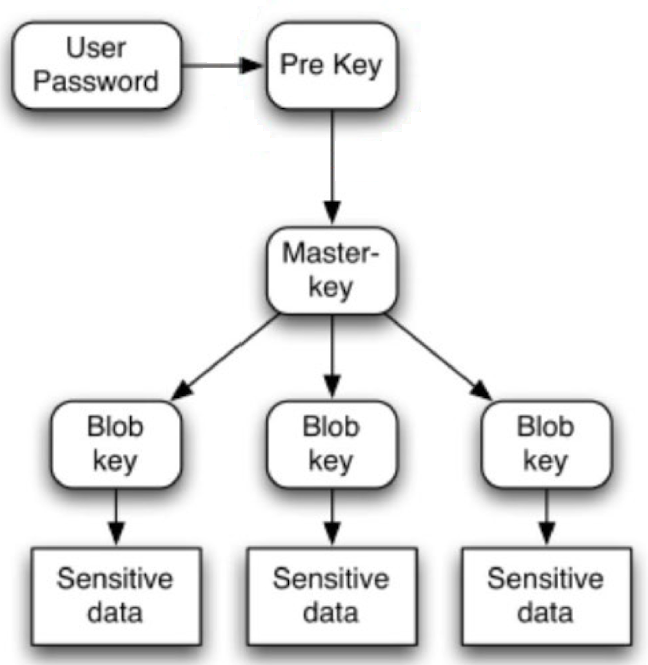
\includegraphics[width=.4\linewidth]{./img/05-mimikatz/dpapi_master_key}
    \vspace{-8pt}
\end{center}

\subsubsection{decrypt User Secrets}
DPAPI-Benutzer-Masterkeys befinden sich im LSASS-Speicher für angemeldete Benutzer. Im Kontext eines Benutzers ist die einfachste Entschlüsselungsmethode für viele (aber nicht alle) DPAPI Blobs, CryptUnprotectData() aufzurufen, damit das Betriebssystem den Blob entschlüsselt.

\subsubsection{get the User Master Key}
Um DPAPI-Datenblöcke OHNE Verwendung der etablierten APIs zu entschlüsseln wird der SHA1 des entschlüsselten Masterkeys benötigt. Kann mit Mimikatz aus LSASS gelesen werden.

\subsubsection{decrypt Machine Secrets}
Zum Entschlüsseln von Machine Secrets wird das DPAPI\_SYSTEM LSA Secret benötigt. Dieser Schlüssel kann dann verwendet werden, um die Hauptschlüssel der Maschinen zu entschlüsseln.

\subsubsection{Credentials, Vaults, .rdg, Chrome, ...}
Credentials werden im Credentials-Ordnern aufbewahrt: in sich geschlossene Strukturen\\
Vaults werden in Vaults-Ordnern aufbewahrt, haben eine Policy.vpol, die mit einem Hauptschlüssel entschlüsselt wird, zwei AES Schlüssel innerhalb der Richtlinie werden dann zur Entschlüsselung einer oder mehrerer .vcrd-Dateien verwendet.\\
Mimikatz kann diese entschlüsseln (mit SHA1 des Masterkeys).

\subsection{Credential Abuse Countermeasures}
\subsubsection{Was KB2871997 macht (Verbesserung von Microsoft)}
Neben anderen Verbesserungen zur Verringerung des Risikos von Pass-the-Hash-Angriffen wird die Art und Weise verbessert, wie Windows Anmeldedaten behandelt, z. B:
\begin{itemize}
    \item Beschränkung des Zwischenspeichers für Anmeldeinformationen auf die Lebensdauer der Anmeldung
    \item Beschränkung des Zwischenspeichers für von Kerberos/NTLM/Digest/CredSSP bereitgestellte Anmeldeinformationen
    \item Kerberos-Zwischenspeicher für Klartextkennwörter einschränken
    \item keine Anmeldedaten in CredSSP zwischenspeichern
    \item Verwendung von Anmeldeinformationen für Digest einschränken
\end{itemize}

\subsubsection{Countermeasures Zusammenfassung}
\begin{itemize}
    \item Keine Wiederverwendung von Passwörtern
    \item Verwendung von sicheren Passwörtern und Schutz von Hashes
    \item Implementieren Sie Anmeldebeschränkungen für Ihre privilegierten Konten, um die Gefährdung zu begrenzen
    \item Implementieren Sie ein Active Directory-Verwaltungsschichtmodell
    \item Nutzen Sie die Gruppe "Geschützte Benutzer" in Windows AD
\end{itemize}


\subparagraph{Mimikatz}
% -------- Gian flütsch content --------
\subsubsection{What is the use case of mimikatz}
Mimikatz is a open source program for Microsoft Windows that can be used to display cached credentials by exploiting vulnerabilities.

\subsubsection{What does it mean to get the NTLM hash of John Doe. Is this a problem?}
The \textit{NTLM} hash is a cryptographic hash function. It is used by the Microsoft LAN Manager and partly by Windows NT-based operating systems to store 128-bit hash values of passwords.

With mimikatz, the \textit{NTLM} as well as the \textit{SHA1} hash and other information can be read out relatively easily using the command \lstinline|sekurlsa::logonpasswords|. Furthermore, even the password of the created user is visible in plain text. It is therefore very easy to obtain the password or the \textit{NTLM} hash.

\subsubsection{Pass-the-Hash attack}
\textit{Pass-the-hash} is an attack method that uses the hash value of a password to authenticate against a system. Through vulnerabilities in the system or in the authentication protocols, the hash value can be read out with tools and used for authentication.

Typically, with \textit{pass-the-hash}, you use an NT hash from a compromised user account to authenticate directly as that user to remote services, either by injecting it into the current Windows user's memory or by passing the hash directly to client applications that accept it.

Pass the hash (PtH) is a method of authenticating as a user without having access to the user's cleartext password. This method bypasses standard authentication steps that require a cleartext password, moving directly into the portion of the authentication that uses the password hash. In this technique, valid password hashes for the account being used are captured using a Credential Access technique. Captured hashes are used with PtH to authenticate as that user. Once authenticated, PtH may be used to perform actions on local or remote systems.

\subsubsection{Pass-the-Ticket attack}
\textit{Pass-the-ticket} attacks target Kerberos in a similar way to golden ticket and silver ticket attack. However, in \textit{pass-the-ticket} attacks, an attacker does not forge Kerberos tickets. Instead, they steal valid tickets that have already been created and issued and pass them from one system to another to access resources as a legitimate, privileged user.

\subsubsection{Over-Pass-the-Hash (Pass-the-Key) attack}
The \textit{overpass-the-hash} attack works similarly to the pass-the-hash attack, but takes this technique one step further to obtain a valid Kerberos ticket.

With \textit{overpass-the-hash}, you can use this NT hash twice to now request a full Kerberos GTT or service ticket from the KDC on behalf of this compromised user. This technique also opens up the "pass-the-ticket" attack vector, where the forged but valid (before the expiry date) TGT/ST can now be exported and re-injected for future use, bypassing communication with the KDC.

\subsubsection{Kerberos Golden Ticket attack}
A \textit{golden ticket} attack allows an attacker to create a Kerberos authentication ticket from a compromised service account.

Using the hash of this compromised account and some information about the domain, an attacker can create fraudulent tickets. These tickets appear to be pre-authorized to perform any action the attackers wish without real authentication.

This attack is stealthy and difficult to detect, making it attractive to attackers who plan to live in a domain for a while.

\subsubsection{Kerberos Silver Ticket attack}
A \textit{silver ticket} attack is similar in concept to a golden ticket and involves compromising credentials and abusing the design of the Kerberos protocol. However, unlike a golden ticket, which gives an attacker unrestricted access to the domain, a \textit{silver ticket} only allows an attacker to forge ticket-granting service (TGS) tickets for specific services. TGS tickets are encrypted with the password hash for the service - so if an attacker steals the hash for a service account, they can forge TGS tickets for that service.

While the scope may be smaller, it is still a powerful tool in an attacker's kit, providing persistent and stealthy access to resources. Since only the password hash of the service account is needed, it is also much easier to execute than a golden ticket.

\subsubsection{Pass-the-Cache attack}
A \textit{Pass-the-Cache} attack is generally the same as Pass-the-Ticket, but using the stored and encrypted credentials in a Mac/UNIX/Linux system.

This technique allows an attacker to replay Kerberos credentials compromised from a Linux system to Windows systems within an Active Directory domain.

\subparagraph{Sysmon}

\subsubsection{Explain the purpose of sysmon}
\textit{Sysmon} is a Windows system service and device driver that, once installed on a system, remains resident across system reboots to monitor system activity and log it to the Windows Event Log. It provides detailed information on process creation, network connections and file creation time changes. By collecting the events it generates using the Windows Event Log and then analysing them, you can identify malicious or anomalous activity and understand how intruders and malware operate on your network.

\subsubsection{Explain how and why sysmon is able to detect mimikatz}
Mimikatz requires the privilege \lstinline|privilege::debug| , as it interacts with processes such as \textit{LSASS}. This activity can be detected by focusing on all Sysmon events that have Event ID 10 and where the target process is listed as \lstinline|C:\Windows\system32\lsass.exe|.\\

But this question is answered very well on Medium and is therefore quoted below with reference to the source.\\

\textbf{Using Sysmon to detect command line execution:}\\
Before attackers can execute Mimikatz and dump Windows credentials, they must first download the binary into your environment. Sysmon Event ID 1 tracks Windows process creation and shows the command line execution used to invoke shell processes.\\

\textbf{Using Sysmon To Detect Obfuscated Command Line Execution}\\
Threat actors will often obfuscate their command line execution in order to evade endpoint detection. Base64 encoding is a common adversarial obfuscation tactic.\\

\textbf{Using Sysmon To Detect Mimikatz Accessing Lsass Memory}\\
The lsass process enforces the Windows security policy, verifies user logons, and handles user password changes. If you configure sysmon to watch for Mimikatz accessing the lsass process, sysmon Event ID 10 will show Mimikatz behaving as a parent process and accessing lsass.exe, behaving as a child process.

By adding the following setting to the sysmon Config, the detection of access to the LSASS process can be further improved:

\begin{lstlisting}[language=XML]
    <!--SYSMON EVENT ID 10 : INTER-PROCESS ACCESS-->
    <!--DATA: UtcTime, SourceProcessGuid, SourceProcessId, SourceThreadId, SourceImage, TargetProcessGuid, TargetProcessId, TargetImage, GrantedAccess, CallTrace-->
    <ProcessAccess onmatch="include">
        <TargetImage condition="contains">lsass.exe</TargetImage>
    </ProcessAccess>
\end{lstlisting}

\subsubsection{Would it be possible to log an event where a victim user would start a dangerous makro embedded in a Word file that would execute a power shell script?}
Yes, it is possible to detect such macros.\\
The following query is necessary to detect word files with embedded macros opened via outlook:\\
\begin{itemize}
    \item \lstinline|`event_data.ParentImage: outlook.exe AND event_data.CommandLine: ".doc"`| (sysmon Event ID: 1)
    \item \lstinline|`event_data.Image: outlook.exe AND event_data.TargetFilename: ".doc"`| (sysmon Event ID: 15)\\
\end{itemize}

In addition, the following sysmon configuration can be used to create an event for each \textit{Protect Document Editing} or \textit{Activate Macros} (sysmon Event ID: 13).

\begin{lstlisting}[language=XML]
    <Sysmon schemaversion="4.00">
        <HashAlgorithms>md5,sha256</HashAlgorithms>
        <EventFiltering>
            <RegistryEvent onmatch="include">
                <TargetObject condition="contains">
                    Security\Trusted Documents\TrustRecords
                </TargetObject>
            </RegistryEvent>
        </EventFiltering>
    </Sysmon>
\end{lstlisting}

\subsubsection{If you reboot/restart the Windows 10 VM, do you need to run sysmon again?}
No. Once sysmon is installed, is remains resident across system reboots to monitor system activity

\subsubsection{Sysmon rules are organized by Event IDs. Which Event ID is most interesting for detecting mimikatz?}
This activity can be detected by focussing on any sysmon events that have the event ID of 10 and where the target process is listed as \lstinline|C:\Windows\system32\lsass.exe| and \lstinline|GrantedAccess| is \lstinline|0x1010|.

\subsubsection{Would it be possible to flag the mimikatz detection as alarm in the Event Viewer?}
According to my research, I have not found anything where Event Viewer alerts can be created via sysmon. All detections from sysmon are displayed in the Event Viewer as \textit{Information}\color{black} and the critical messages can then be filtered via the \textit{event ID}.

\subsubsection{Explain the idea of sigma rules}
Sigma Rules are a generic and open signature format that allows to describe relevant log events in a straight forward manner. The rule format is very flexible, easy to write and applicable to any type of log file. The main purpose of sigma rules is to provide a structured form in which researchers or analysts can describe their once developed detection methods and make them shareable with others.

\subsubsection{Explain how sigma rules could be beneficial with sysmon}
With sigma rules, previously unknown mimikatz attacks can be mapped and integrated into Sysmon for detection.
